% !TEX root = ../main.tex
\graphicspath{ {./figures/} }

%%%%%%%%%%%%%%%%%%%%
\chapter{Evaluation}
\label{chap:evaluation}
%%%%%%%%%%%%%%%%%%%%

The three solvers will be evaluated based on their runtime and scalability. The evaluation will first cover synthetically generated delegation graphs including randomly generated small and big graphs as well as corner cases, then delegations graphs generated based on social behaviors, so-called social graphs, and finally graphs based on real-world datasets.

\section{Method}

\subsection{Generating Random Delegation Graphs}

For \cref{sec:synthetic_graphs} on synthetically generated graphs we built an algorithm, that builds custom delegation graphs. The algorithm generates an empty graph with $n$ nodes, and then adds between zero and three delegations per node to random other nodes, ensuring that there are no closed delegation cycles. A better explanation of how these graphs are artificially constructed can be found in the Annex. \TODO{Create this annex} We acknowledge that these assumptions may not accurately reflect real-world delegation graphs. Studies have shown that delegates do not choose randomly; instead, votes often concentrate among a few individuals. This approach also overlooks behavioral tendencies, such as voters preferring to delegate to those they perceive as more competent or confident, and the emergence of highly popular "super-voters" who accumulate disproportionate influence. \cite{klingVotingBehaviourPower2015} These concerns are addressed in \cref{sec:social_graphs}, when delegation graphs based on social graphs are benchmarked. 

\subsection{Preprocessing}

In order to be able to benchmark algorithms that resolve delegations, the input graphs need to be well-formed delegation graphs. Many of the graphs we use for benchmarking are not well-formed delegation graphs out-of-the-box. This subsection details the process of how any arbitrary graphs, including undirected and unweighted graphs, can be turned into well-formed delegation graphs. An overview of this process is shown in \cref{fig:cleaning_process}.

\begin{figure}[t]
    \centering
    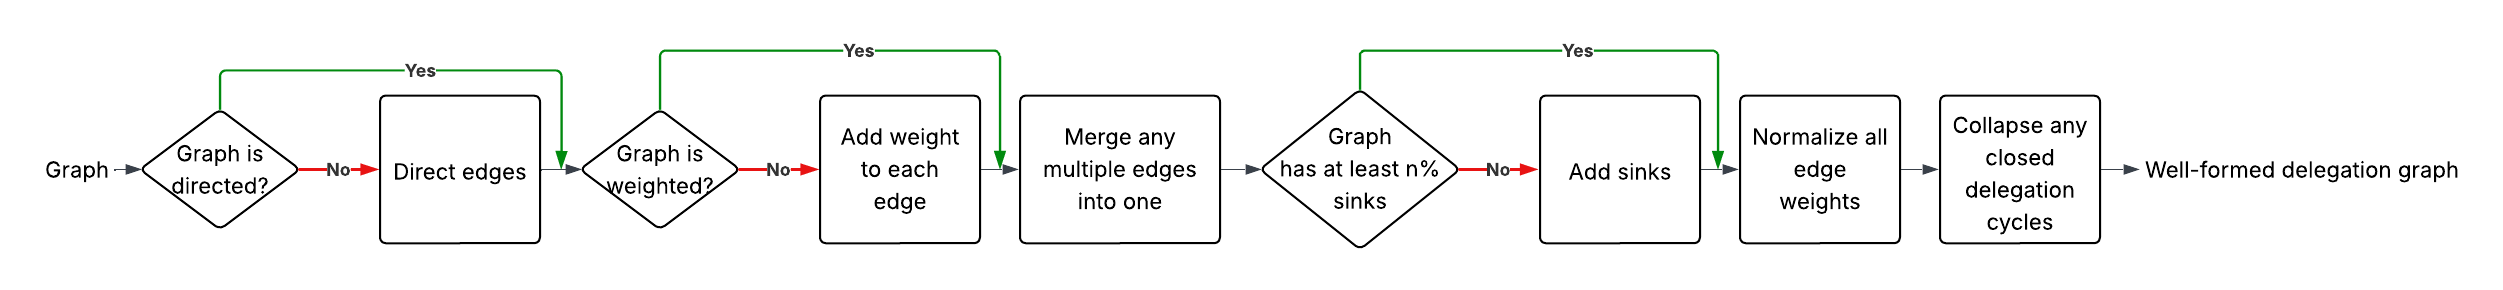
\includegraphics[width=\textwidth]{Thesis Evaluation Methodology Process.png}
    \caption{Preprocessign pipeline to turn any graph into a delegation graph}
    \label{fig:cleaning_process}
\end{figure}

If the graph is undirected, is it given a direction. This is done arbitrarily, with the algorithm interpreting undirected edges in the shape $(u, v)$ as directed edges from u to v. If the algorithm fails to find a weight for an edge, it will also assign it a weight of one. Next, any multiple edges, so parallel edges going from the same node to the same node are merged, with any weights being added together. If less than $n\%$ of the graph's nodes are sinks, the algorithm randomly removes all outgoing delegations of delegators, turning them into sinks. By default this n value is 20, however depending on the use case it can be increased or decreased. After this, the algorithm searched for any closed delegation cycles, and collapses all it finds into a single sink node. Specifically, the algorithm searched for strongly connected components (STCCs) in the graph, so components of the graph where each node can reach each other node, and checks if it it is a closed delegation cycle, by checking if any of the nodes within this STCC to a node outside of the STCC. An exception to this are sinks who have no delegators, these are technically STCCs with no outgoing edges, however they are not closed delegation cycles. All closed delegation cycles are collapsed into a "lost" node, which means that any delegations to the cycle get re-directed to a specially created node. The resulting graph from this operation is a well-formed delegation graph, since all power that flows into closed delegation cycles now flows into a sink, so the graph is free of closed delegation cycles.

\subsection{Measurement}

Despite all algorithm's taking in put in inverse dict-of-dicts format, there may still be preprocessing necessary. While the iterative solver can use the inverse dict-of-dicts directly, using it as a lookup table as it spreads power around the graph, the other solver require the system of linear equations in specific formats, which need to be set up from the inverse dict-of-dicts input. Including such set-up time in benchmarks may be misleading, as this time is not spent on actually resolving delegations, thus we separated the set-up and resolving, and in the benchmarks only the time spent actually resolving the delegations is used; any set-up time is ignored. Nevertheless, in practice, the set-up time can be a relevant factor—depending on the use case and data format—when choosing between different approaches or implementations. The set-up procedures required for each implementation are described in more detail in the sections below.

To minimize the impact of background noise and measurement fluctuations on the benchmarks, algorithms with very short runtimes were executed multiple times, and the average runtime was recorded. The recorded runtimes always indicate just the runtime for the algorithms to resolve the delegations, times for set-up, such as the time for building the linear program, are not included. 

Furthermore, all runtimes are reported based on the actual number of nodes present in the resolved graph. For example, if a delegation graph initially contains $5000$ nodes, but $500$ of are in closed delegation cycles, these are collapsed into a single sink node. 
When the algorithm is thus resolving the graph, all of these $500$ nodes are in effect just one node. Thus, when presenting benchmarks results, for this graph, we will show the amount of nodes resulting in the presented runtime as $4501$. 

\section{Synthetic Graphs}
\label{sec:synthetic_graphs}

\subsection{Small Graphs}
\label{subsec:small_graphs}

\begin{figure}[t]
    \centering
    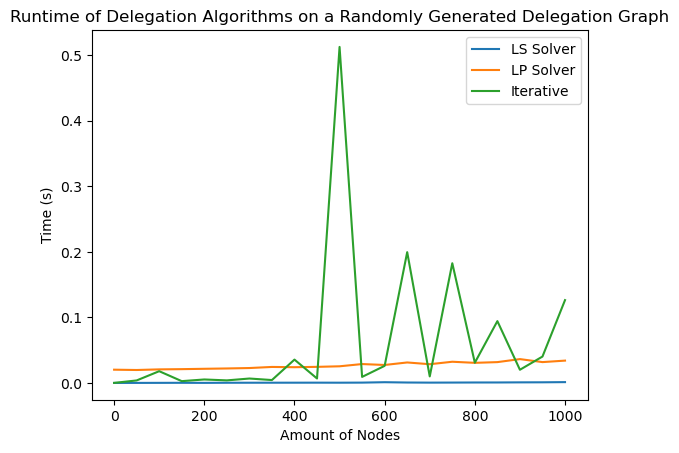
\includegraphics[width=0.4\textwidth]{0-1000_random}
    \caption{Runtime of delegation algorithms on a randomly generated delegation graph}
    \label{fig:random-small}
\end{figure}

In order to explore the three algorithm's behavior on small graphs, we used the graph generator to generate graphs with zero to 1000 nodes. \Cref{fig:random-small} shows the results of this benchmark.

We see, that the \ac{LS} Implementation, optimized for sparse matrices, outperforms the other two algorithms. Its growth in runtime is so small, that the line looks to be staying flat on the x-axis. However, with a graph of 1000 nodes, its runtime is about 0.002 seconds. Both the LS and LP implementations display a rather steady, yet growing runtime. The LP solver seems to have some overhead, since even when the graph has zero nodes, it has a runtime of about 0.02 seconds.

Furthermore, we can observe large spikes in the runtime of the iterative approach. For example, resolving the delegation graph with 650 nodes takes the algorithm more than double the amount of time than the graph with 700 nodes. Exploring this phenomenon more closely, we find that a graph with 13 nodes takes the iterative algorithm a lot more time than the graph with 12 or 14 nodes, as shown in \cref{fig:random-tiny}. At 12 nodes, the runtime of the iterative algorithm is just about 0.2 milliseconds, at 14 nodes it is about 0.3 milliseconds, but at 13 nodes it is 4.3 milliseconds. 

\begin{figure}[t]
    \centering
    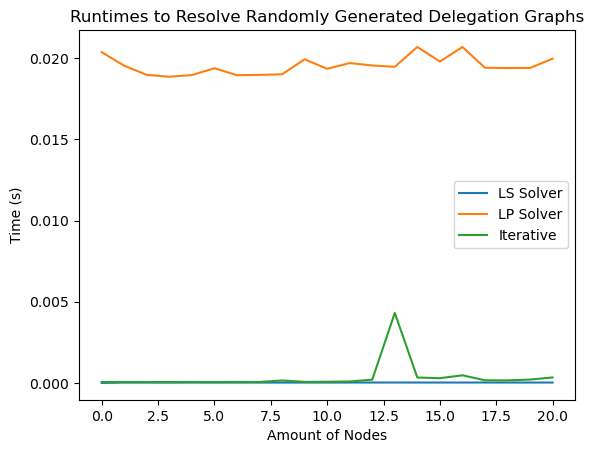
\includegraphics[width=0.4\textwidth]{0-20_random}
    \caption{Runtimes to resolve randomly generated delegation graphs}
    \label{fig:random-tiny}
\end{figure}

A possible explanation for this spike may be, that when the graph has 12 and 14 nodes, it iterates only 23 and 39 times respectively, before cutting off, while when it has 13 nodes it iterates 740 times before cutting off. \Cref{fig:random-12and13} shows the two graphs with 12 and 13 nodes.

\begin{figure}[t]
    \centering
    \begin{subfigure}[t]{0.45\textwidth}
        \centering
        \fbox{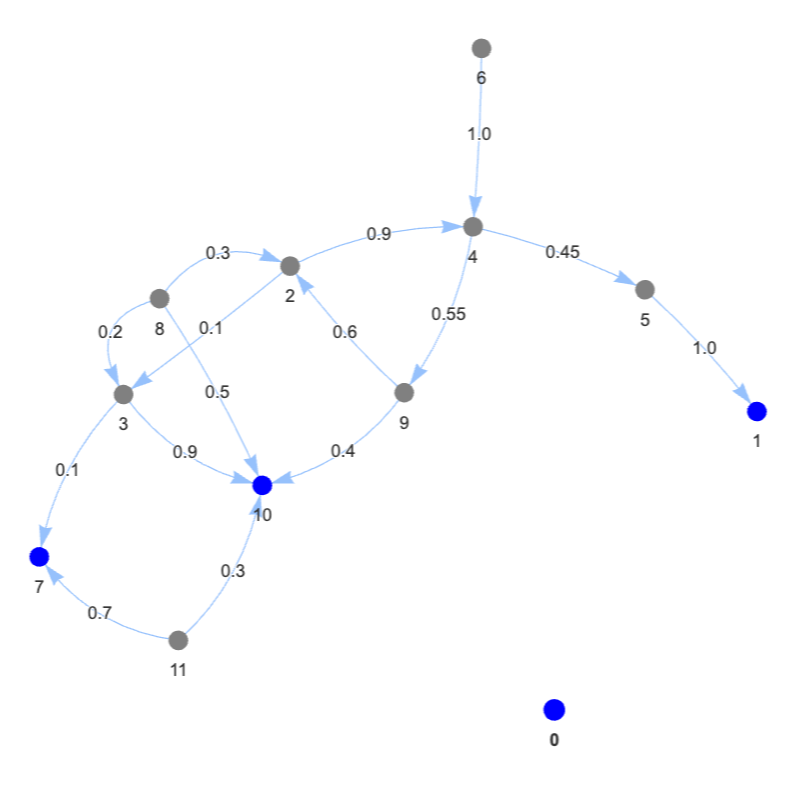
\includegraphics[width=\textwidth]{12_4_random}}
        \caption{12 nodes}
        \label{subfig:random-12and13-12}
    \end{subfigure}
    \hfill
    \begin{subfigure}[t]{0.45\textwidth}
        \centering
        \fbox{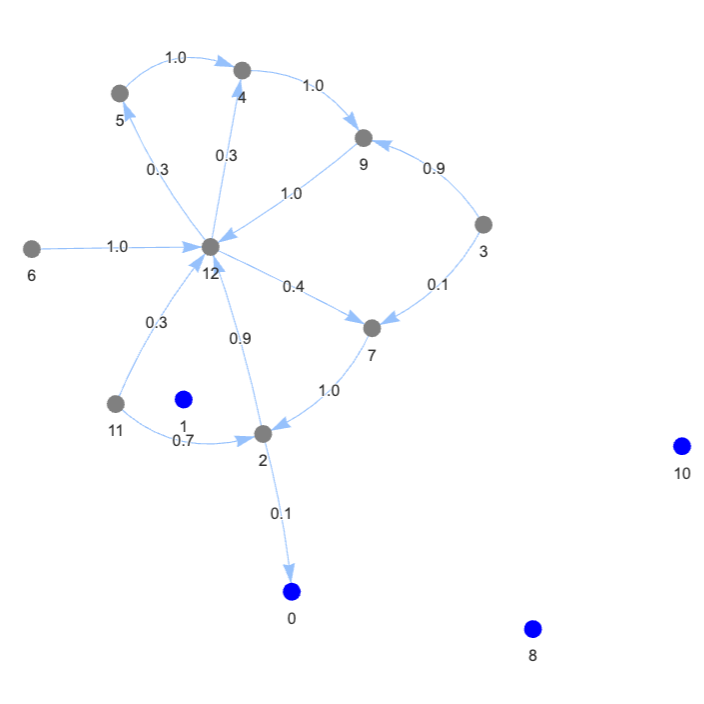
\includegraphics[width=\textwidth]{13_4_random}}
        \caption{13 nodes}
        \label{subfig:random-12and13-13}
    \end{subfigure}
    \caption{Delegation graphs with 12 and 13 nodes (blue nodes are sinks)}
    \label{fig:random-12and13}
\end{figure}

When the graph has 13 nodes, power entering the sink node \texttt{0} only has a delegation of weight 0.1. Each iteration, 10\% of the power within node \texttt{2} enters the sink, but the other 90\% is dispersed into the graph. This forces the iterative algorithm to iterate this power around the graph until eventually enough of it has collected in node \texttt{0}. In the graph with 12 nodes on the other hand, this effect is visibly less present. A delegation from node \texttt{3} to sink node \texttt{7} only has a weight of 0.1 too, but the other 0.9 of this vote are directed toward another sink node \texttt{10}. Furthermore, node \texttt{3} is not in a cycle. 

This is an important shortcoming of the iterative algorithm. Power can easily get trapped within permissible delegation cycles that only have a small drain allowing the power to escape from the cycle. Each iteration, if a great proportion of the nodes with draining edges' power is sent back into a cycle, the algorithm needs to continuously iterate until the power is back at the drain nodes, however depending on the cycle this may happen very inefficiently. This phenomenon will be tested more in \cref{subsec:cycles_draining}

\subsection{Large Graphs}

Delegation graphs may grow arbitrarily large. National elections for example can contains up to hundreds of millions of participants. This section explores how the algorithms perform when having to resolve graphs with a lot of nodes. Again, the graphs will be randomly generated, such that each nodes has between 0 and 3 delegates. 

\begin{figure}[t]

\end{figure}

\begin{figure}[t]
    \centering
    \begin{subfigure}[t]{0.45\textwidth}
    	\centering
    	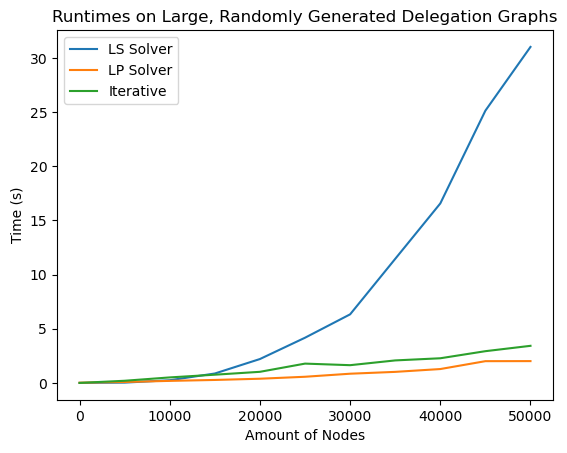
\includegraphics[width=\textwidth]{0-50000_random}
    	\caption{Linear scale}
    	\label{fig:random-large-linear}
    \end{subfigure}
    \hfill
    \begin{subfigure}[t]{0.45\textwidth}
        \centering
        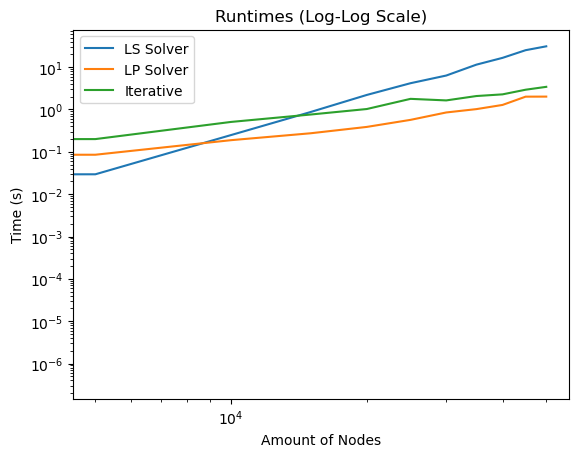
\includegraphics[width=\textwidth]{0-50000_random_loglog}
        \caption{Loglog scale}
         \label{subfig:random-large-loglog}
    \end{subfigure}
    \caption{Runtimes to resolve large, randomly generated delegation graphs}
    \label{fig:random-large}
\end{figure}

\Cref{fig:random-large} shows that even as the delegation graphs get larger, the LS solver's runtime grows faster than that of the other two implementations. For resolving smaller graphs, the LS solver outperforms the LP solver, with a runtime of almost zero for empty or very small graphs, while the LP solver has a clearly non-zero runtime even for very small graphs. However, at around 12 000 nodes, this changes, as the LP solver's runtime's slower growth catches up with that of the LS solver, closely followed by the iterative implementation. 

Looking at the loglog graph, the runtime growths seem to be following a power law. Fitting the data into different curves confirms, that the implementations likely all grow according to a power law, with the LS solver growing the quickest, about $O(n^{3.07})$, $n$ being the amount of nodes, the LP solver fitting into an $O(n^{1.41})$ curve and the iterative solver $O(n^{1.20})$. These growth classes are probably not generalizable to all delegation graphs, since the runtime may grow with different coefficients depending on the underlying delegation graphs. This will be explored in the following sections.


\subsection{Dense Graphs}

While we expect most delegators in any delegation graph to only delegate to a handful of people, a well formed delegation graph can have any number of delegates per delegator. Thus, it is also interesting to compare how the three algorithms compare when resolving more dense graphs. In this section, we test the three implementations on NetworkX's $G_{n,p}$ graph generator \texttt{gnp\_random\_graph}, which returns a directed graph with $n$ nodes, where each node connected to each other node with probability $p$, which is set to $0.5$ for the remainder of this section \cite{hagbergExploringNetworkStructure2008}. All of the nodes in these graphs are not sinks, since they all have outgoing edges. Normally, these graphs would be one large closed delegation cycle, where nobody votes, and the preprocessing pipeline would collapse them all into one sink node. Thus, in order to be able to resolve meaningful power values, we turn 10\% of nodes into sinks by removing the outgoing edges. Then, each delegators vote is equally distributed to all of its outgoing edges, such that the edge weights add up to 1. Finally, any remaining closed delegation cycles are collapsed, however, all graphs that the benchmark was run on ended up having no closed delegations after the measures were applied.

\begin{figure}[t]
    \centering
    \begin{subfigure}[t]{0.45\textwidth}
    	\centering
    	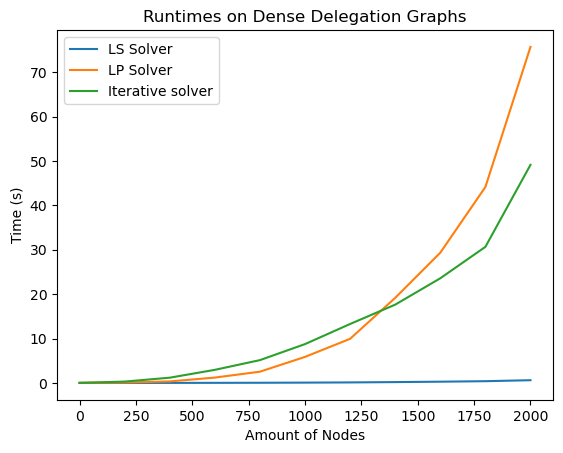
\includegraphics[width=\textwidth]{0-2000_dense}
    	\caption{Linear scale}
    	\label{fig:dense-linear}
    \end{subfigure}
    \hfill
    \begin{subfigure}[t]{0.45\textwidth}
        \centering
        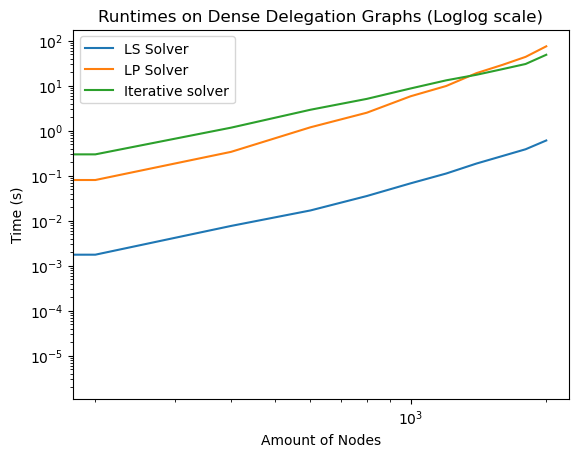
\includegraphics[width=\textwidth]{0-2000_dense_loglog}
        \caption{Loglog scale}
         \label{subfig:dense-loglog}
    \end{subfigure}
    \caption{Runtimes to resolve dense delegation graphs}
    \label{fig:dense}
\end{figure}

\Cref{fig:dense} shows the runtime of these three algorithms. The runtimes are greater than the runtimes found in the previous section. At 2000 nodes, the runtimes on the randomly generated, relatively sparse, graphs was well under a second for each algorithm, while it takes the iterative and LP solver 49 and 76 seconds respectively. The LS solver's runtime grows from about 0.03 to 0.61 to resolve the dense graph. The LS solver surprisingly outperforms both solvers, however looking at its runtime growth in a loglog graph reveals, that is grows at a similar rate to the others. Which algorithm is the slowest depends on the amount of nodes in the graph, with the iterative solver showing slower runtime growth, eventually outperforming the LP solver at around 1300 nodes. The delegations in this graph are very fine grained, since each delegating node delegates to half of all nodes, and the delegators vote is distributed equally to all its delegates, the weight of each delegation is just:

\[ 
\frac{1}{0.5n} = \frac{2}{n} 
\]

Intuitively, this should put the iterative algorithm at a disadvantage, since it needs to iterate around a lot of delegations, each only moving around small amounts of power at a time. However, it seems that the LP implementation struggles with these graphs as well, likely because the large amount of delegations results in lot of long linear equations to solve. Even though the LS solver is optimized for sparse matrices, it demonstrates impressive efficiency at solving these kinds of problems.

\begin{figure}[t]
    \centering
    \begin{subfigure}[t]{0.45\textwidth}
    	\centering
    	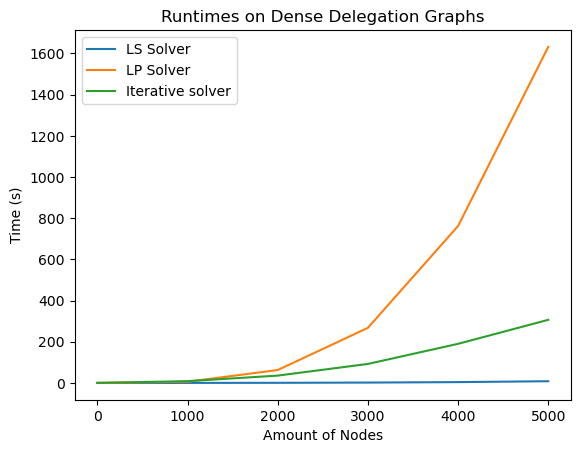
\includegraphics[width=\textwidth]{0-5000_dense}
    	\caption{Linear scale}
    	\label{subfig:dense-large-linear}
    \end{subfigure}
    \hfill
    \begin{subfigure}[t]{0.45\textwidth}
        \centering
        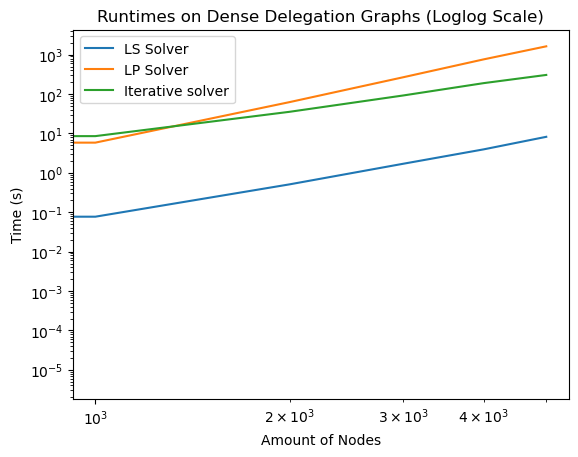
\includegraphics[width=\textwidth]{0-5000_dense_loglog}
        \caption{Loglog scale}
         \label{subfig:dense-large-loglog}
    \end{subfigure}
    \caption{Runtimes to resolve larger dense delegation graphs}
    \label{fig:dense-large}
\end{figure}

Testing the three algorithms on larger dense graphs, reveals that the LP solver's runtime is considerably worse than that of both the iterative and LS solver. A dense graph with 5,000 nodes, takes the LS solver only about eight seconds, the iterative solver 306 seconds, and the LP solver 1632 seconds. Fitting curves on these runtimes again reveals that they likely follow a power law, the runtime classes for the LS, LP and iterative solver being $O(n^{2.89})$, $O(n^{3.51})$ and $O(n^{2.24})$ respectively. As is also visible in \cref{subfig:dense-large-loglog}, this means the iterative algorithm has the best runtime class, however for dense graphs of the size that was tested, it is not the most performant algorithm.

\subsection{Cycles Which Retain a Lot of their Power}
\label{subsec:cycles_draining}

\begin{figure}
\centering
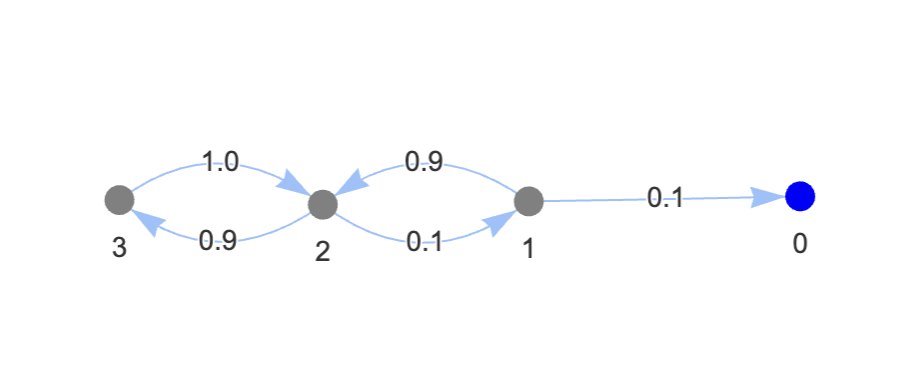
\includegraphics[width=0.40\textwidth]{small_cycle_graph_2}
\caption{A delegation graph with a cycle that retains a lot of its power}
\label{fig:cycle_example}
\end{figure}

To explore one of the iterative algorithm's shortcomings, this section will explore and compare runtime behavior for delegation cycles which are not closed, but contain only few, weak edges for power to drain, thus forcing power to iterate around in the cycle before it reaches a sink. Such situations cause the iterative algorithm's runtime to spike, as has already been observed in \cref{subfig:random-12and13-13}, as the algorithm needs to move around the power within these cycles until enough as drained for the \texttt{max\_change} to fall below the threshold. A further example of such a cycle, motived by graphs which we encountered while experimenting on delegation graphs is the tail-shaped graph in \cref{fig:cycle_example}. 

For the benchmarking, we construct graphs with a circular shape, where delegates all delegate power to the next node in the cycle. One node in the cycle contains an edge with weight 0.1 to a sink, while the other 0.9 of its power goes to the first node in the cycle. \Cref{fig:big_cycle_example} contains an exemplary image of such a graph with 10 nodes. 

\begin{figure}[t]
	\centering
	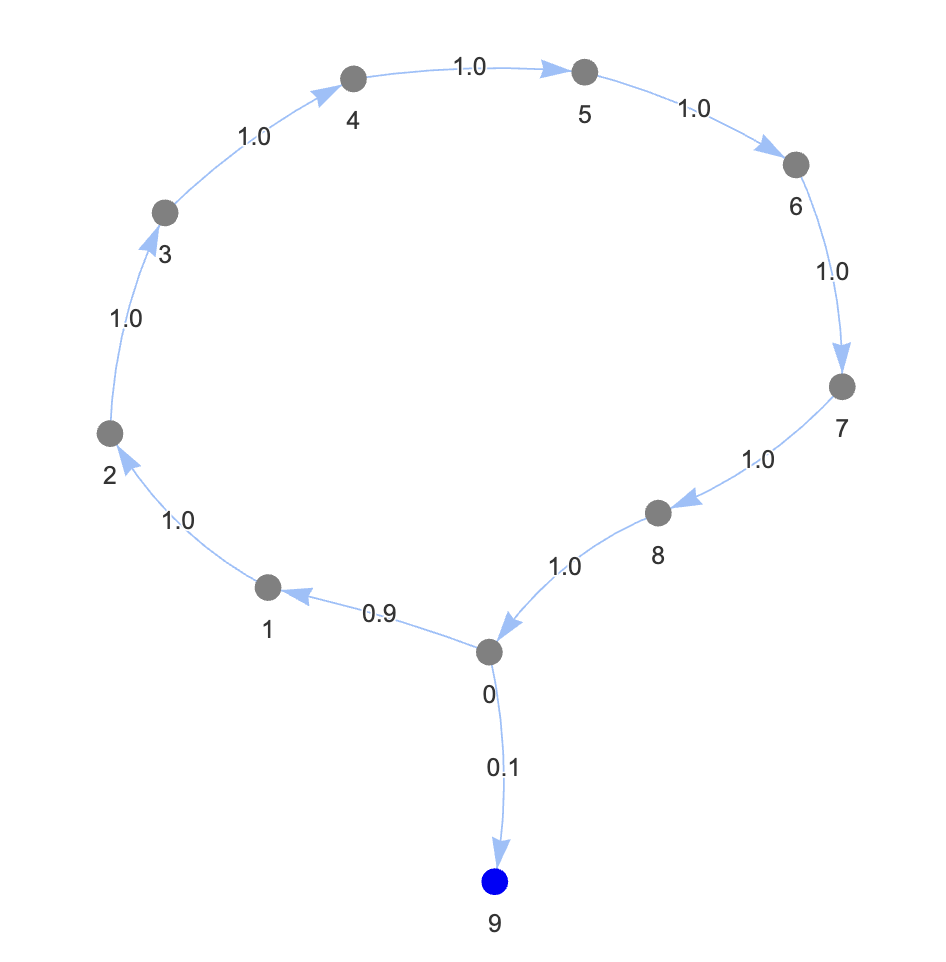
\includegraphics[width=0.4\textwidth]{big_cycle_example}
	\caption{An example of the cycles used for the benchmarks. The blue node is the sink}
	\label{fig:big_cycle_example}
\end{figure}

\begin{figure}[t]
    \centering
    \begin{subfigure}[t]{0.45\textwidth}
    	\centering
    	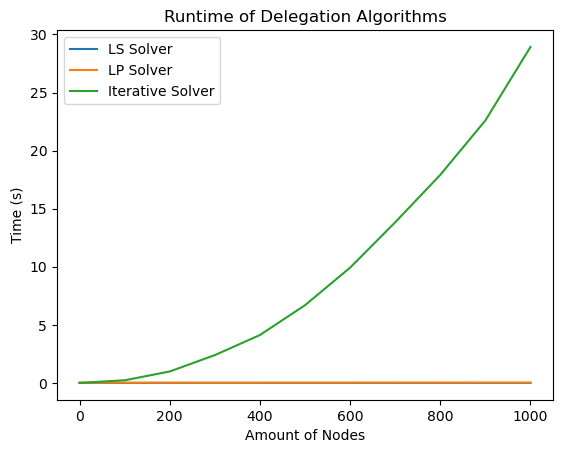
\includegraphics[width=\textwidth]{0-1000_cycle}
    	\caption{Linear scale}
    	\label{subfig:cycle-small-linear}
    \end{subfigure}
    \hfill
    \begin{subfigure}[t]{0.45\textwidth}
        \centering
        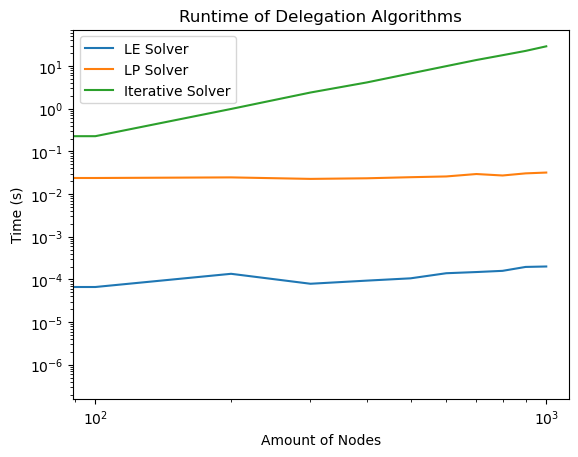
\includegraphics[width=\textwidth]{0-1000_cycle_loglog}
        \caption{Loglog scale}
         \label{subfig:cycle-small-loglog}
    \end{subfigure}
    \caption{Runtimes to resolve cycles which retain a lot of their power}
    \label{fig:cycle_small}
\end{figure}

The runtimes in \cref{subfig:cycle-small-linear} show, that as expected, the iterative algorithm struggles considerably with the resolution of these graphs, while the other two algorithms exhibit behavior similar to that on randomly generated sparse delegation graphs. The growth of the runtimes seems to be polynomial, with the iterative algorithm belonging to the runtime class $O(n^{2.12})$. Being able to resolve these kinds of loops is one of the greatest strength of the two approaches, which don't simulate power as flow through the graph. By directly solving the system of linear equations, they better equipped to deal with this corner case.  

\begin{figure}[t]
    \centering
    \begin{subfigure}[t]{0.45\textwidth}
    	\centering
    	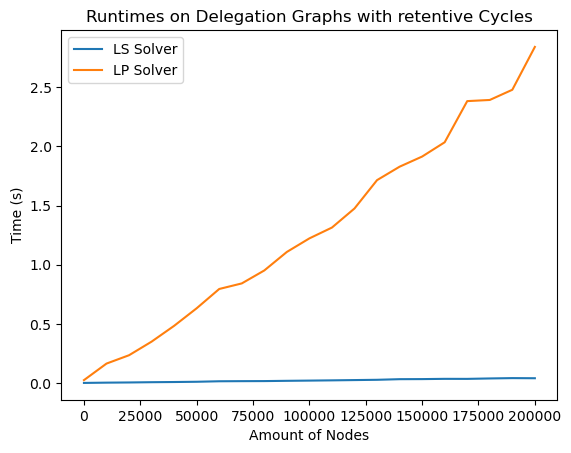
\includegraphics[width=\textwidth]{0-200000_cycle}
    	\caption{Linear scale}
    	\label{subfig:cycle-large-linear}
    \end{subfigure}
    \hfill
    \begin{subfigure}[t]{0.45\textwidth}
        \centering
        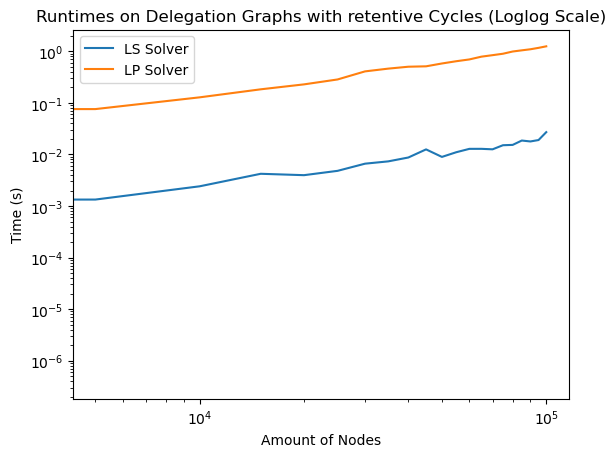
\includegraphics[width=\textwidth]{0-200000_cycle_loglog}
        \caption{Loglog scale}
         \label{subfig:cycle-large-loglog}
    \end{subfigure}
    \caption{Runtimes to resolve cycles which retain a lot of their power. The iterative solver's runtime, to allow inspection of the LS and LP solver's runtimes.}
    \label{fig:cycle_large}
\end{figure}

As seen in \cref{fig:cycle_large}, which shows the LS and LP solver's runtimes as this type of graph scales to $200 000$ nodes, their runtime growth is linear. In fact, they fit almost perfectly into a linear regression, both with a slope of almost zero, suggesting that even as these graphs scale to even greater orders of magnitude, the solver's runtime is barely affected. An explanation for this efficiency may include the very sparse nature of this graph, as each node except for one has only one delegation.

\TODO{Maybe a graph for the real world models, that shows the runtime as precision for the iterative thing increases would be very cool.}

\subsection{No Delegations}

The runtime of the implementations on delegation graphs where all nodes have no outgoing edges can also provide insight, such as the runtime behavior on graphs where only few nodes delegate, or delegations are very short. \Cref{fig:no_del} shows how long it takes for the implementations to resolve graphs which have no edges at all. 

\begin{figure}[t]
    \centering
    \begin{subfigure}[t]{0.45\textwidth}
    	\centering
    	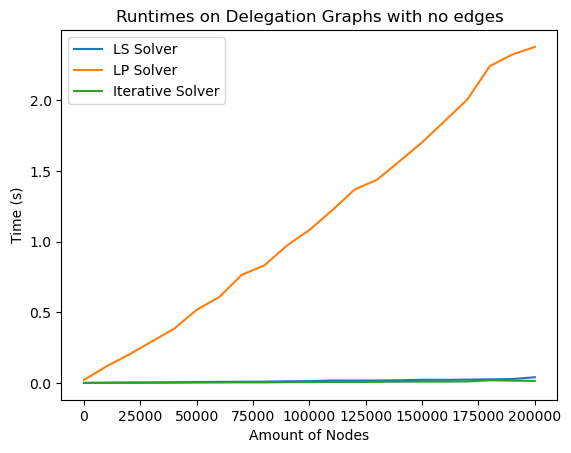
\includegraphics[width=\textwidth]{0-200000_no_del}
    	\caption{Linear scale}
    	\label{subfig:no-del-linear}
    \end{subfigure}
    \hfill
    \begin{subfigure}[t]{0.45\textwidth}
        \centering
        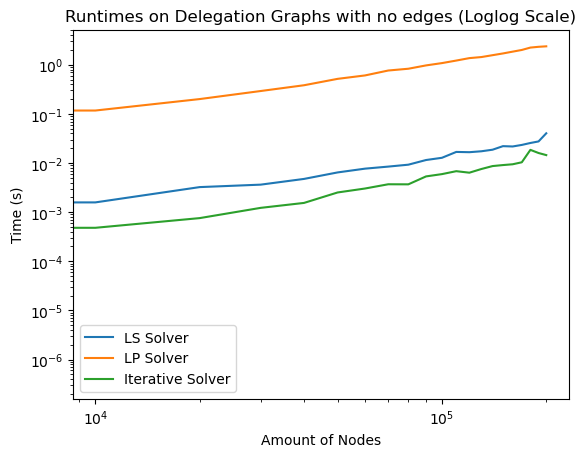
\includegraphics[width=\textwidth]{0-200000_no_del_loglog}
        \caption{Loglog scale}
         \label{subfig:no-del-loglog}
    \end{subfigure}
    \caption{Runtimes to resolve delegation graphs with no edges}
    \label{fig:no_del}
\end{figure}


The iterative algorithm outperforms the other two on these graphs, which is not surprising, since it only needs to iterate over the empty dict of delegations once, registers a \texttt{max\_change} of zero, and terminates. All three solvers' runtimes seem to grow about linearly, where even at 200 000 nodes, the slowest solver, the LP solver, takes only about 2.5 seconds, suggesting they grow linearly with a slope close to one. A linear regressions confirms this observation. 

\section{Social Graphs}
\label{sec:social_graphs}

Social graphs provide an excellent way to create scalable models of trust within communities without real datasets. We will use them to create sample delegation graphs based on social behaviors, which can predict ways humans may delegate if given the chance to delegate fractionally. These graphs are only based on models, however since they are artificial, we can scale them and explore how the algorithms scale.

\subsection{Small World Graphs}

Small world graphs are graph which exhibit a relatively high clustering coefficient, meaning nodes are very interconnected, with short path lengths between arbitrary nodes. Watts and Strogatz propose a graph generator to generate these kinds of graphs artificially. The graph generator takes three parameters $n$, $k$, and $p$. It connects each of the $n$ nodes with $k$ of their neighbors, and once this is done, "rewires" each edge to a different node with probability $p$. Watts and Strogatz recommend a value for $p$ of around $0.1$, to get the two desired qualities of a small world graph: short path lengths between all nodes and high "cliqueness", meaning if two nodes a friends, their respective friends are also likely to be friends with eachother. Furthermore, they suggest that $k >> ln(n)$ in order to guarantee that the graph is connected. 

The graphs as they are recommended by Watts and Strogatz are not usable as delegation graphs. Firstly, no node in this graph is a sink, since each node has $k$ outgoing edges. Secondly, each node has too many, a lot more than $ln(n)$, delegates. This is does not scale. In a graph with e.g. $10 000$ nodes, each node would delegate to almost ten people, and as the graph grows this number increases. Normally we would not expect the total size of the graph to have a very big effect on the amount of delegations per person, since delegation of votes is a personal, individual question. Thus, we adapt these Watts-Strogatz graph generation graphs in the following ways.

\begin{enumerate}
\item Each node is connected to its exactly $k=4$ neighbors. 
\item $60\%$ of the edges in this graph are removed. 
\item Finally, as the graphs get preprocessed in the preprocessing pipeline, we enforce that $20\%$ of the nodes in this graph are sinks my removing outdoing edges of nodes.  
\end{enumerate}

This way, we assume that each node has four trusted friends, but of these trust relationships, only $40\%$ are strong enough for the nodes to want to let their friend vote for them. The value of $20\%$ is a middle ground between observations which will be made in the following sections, where some social graphs have a lot more than $20\%$ sinks, while other have a lot less. The $p$ of $0.1$ thats Watts and Strogatz recommend is kept. A sample of how a graph generated with way is shown in \cref{fig:ws_example}. 

\begin{figure}
\centering
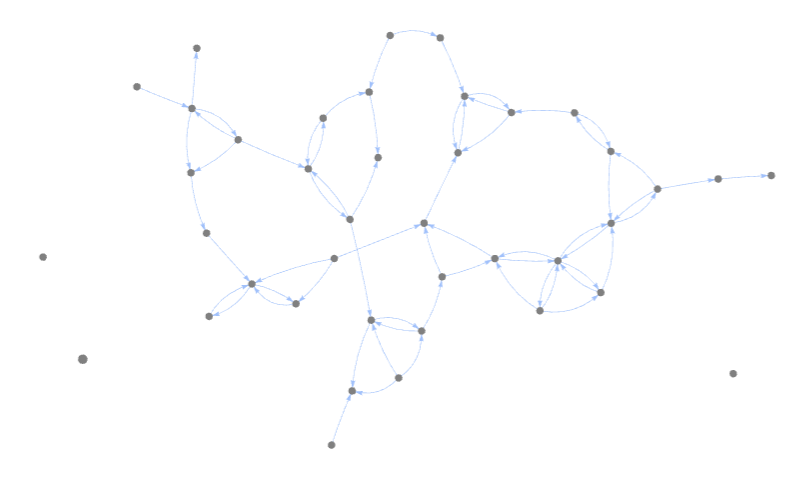
\includegraphics[width=0.40\textwidth]{sw_graph_example_40n.png}
\caption{A Watts-Strogatz graph with $(n, k, p) = (40, 4, 0.1)$, where $60\%$ of the edges have been removed}
\label{fig:ws_example}
\end{figure}

\begin{figure}[t]
    \centering
    \begin{subfigure}[t]{0.45\textwidth}
        \centering
        \fbox{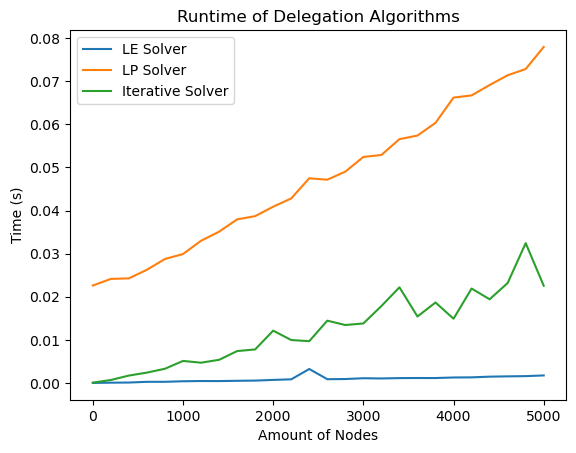
\includegraphics[width=\textwidth]{0-5000_small_world}}
        \caption{Linear scale}
        \label{subfig:sw_linear}
    \end{subfigure}
    \hfill
    \begin{subfigure}[t]{0.45\textwidth}
        \centering
        \fbox{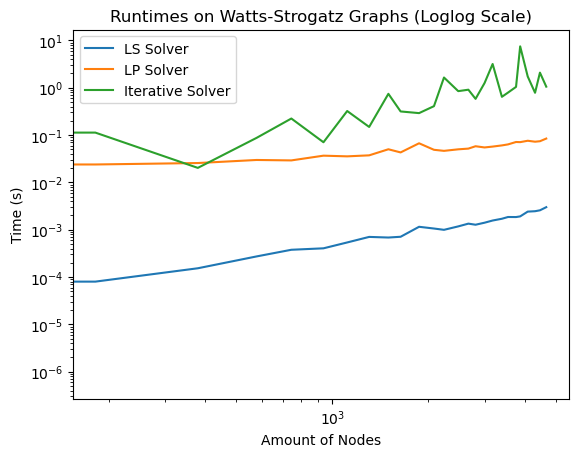
\includegraphics[width=\textwidth]{0-5000_small_world_loglog}}
        \caption{Loglog scale}
        \label{subfig:sw_loglog}
    \end{subfigure}
    \caption{Runtimes to resolve the Watt-Strogatz based delegation graphs. The grey line indicates the amount of cycles found in the graph. It does not include closed delegation cycles, which the preprocessing pipeline collapsed.}
    \label{fig:sw}
\end{figure}




\Cref{fig:sw} shows the benchmarks for these graphs. They are similar to the results achieved when benchmarking the big cycle graphs, where the LS and LP solvers perform quite well compared to the iterative solver. The iterative solver also has a lot rather unpredictable peaks. Investigating this pattern reveals, that even despite our measures, the graphs still contained a lot of (permissible) cycles, so cycles which the direct solvers can solve, but where the iterative algorithm needs to iterate power around the loops. Since there is bit of randomness involved in the creation of these graphs, it can happen that those cycles vary starkly in retentiveness, so the amount of power they force the algorithm to re-loop through a cycle, which leads to peaks and troughs in the iterative solver's runtime. 
 
\TODO{Maybe I still need to revamp this sentence on other sections having more than 20\% sinks}

\subsection{R-Mat Graphs}

Another method for generating artificial social graphs is the R-MAT (Recursive Matrix) model. \cite{chakrabartiRMATRecursiveModel2004} This model requires four parameters—$a$, $b$, $c$, and $d$—which are probabilities that sum to one, as well as the desired number of nodes $N$ and edges $M$. The algorithm begins with an empty $\sqrt{N} \times \sqrt{N}$ adjacency matrix, where a nonzero entry at position $(i, j)$ indicates a directed edge from node $i$ to node $j$. To determine where to place each edge, the matrix is recursively subdivided into four quadrants, with the probability of selecting a quadrant governed by the parameters $a$, $b$, $c$, and $d$. This recursive partitioning continues until a single cell ($1 \times 1$) is reached, and an edge is added at that location. The process is repeated until all $M$ edges have been assigned.

\begin{figure}
\centering
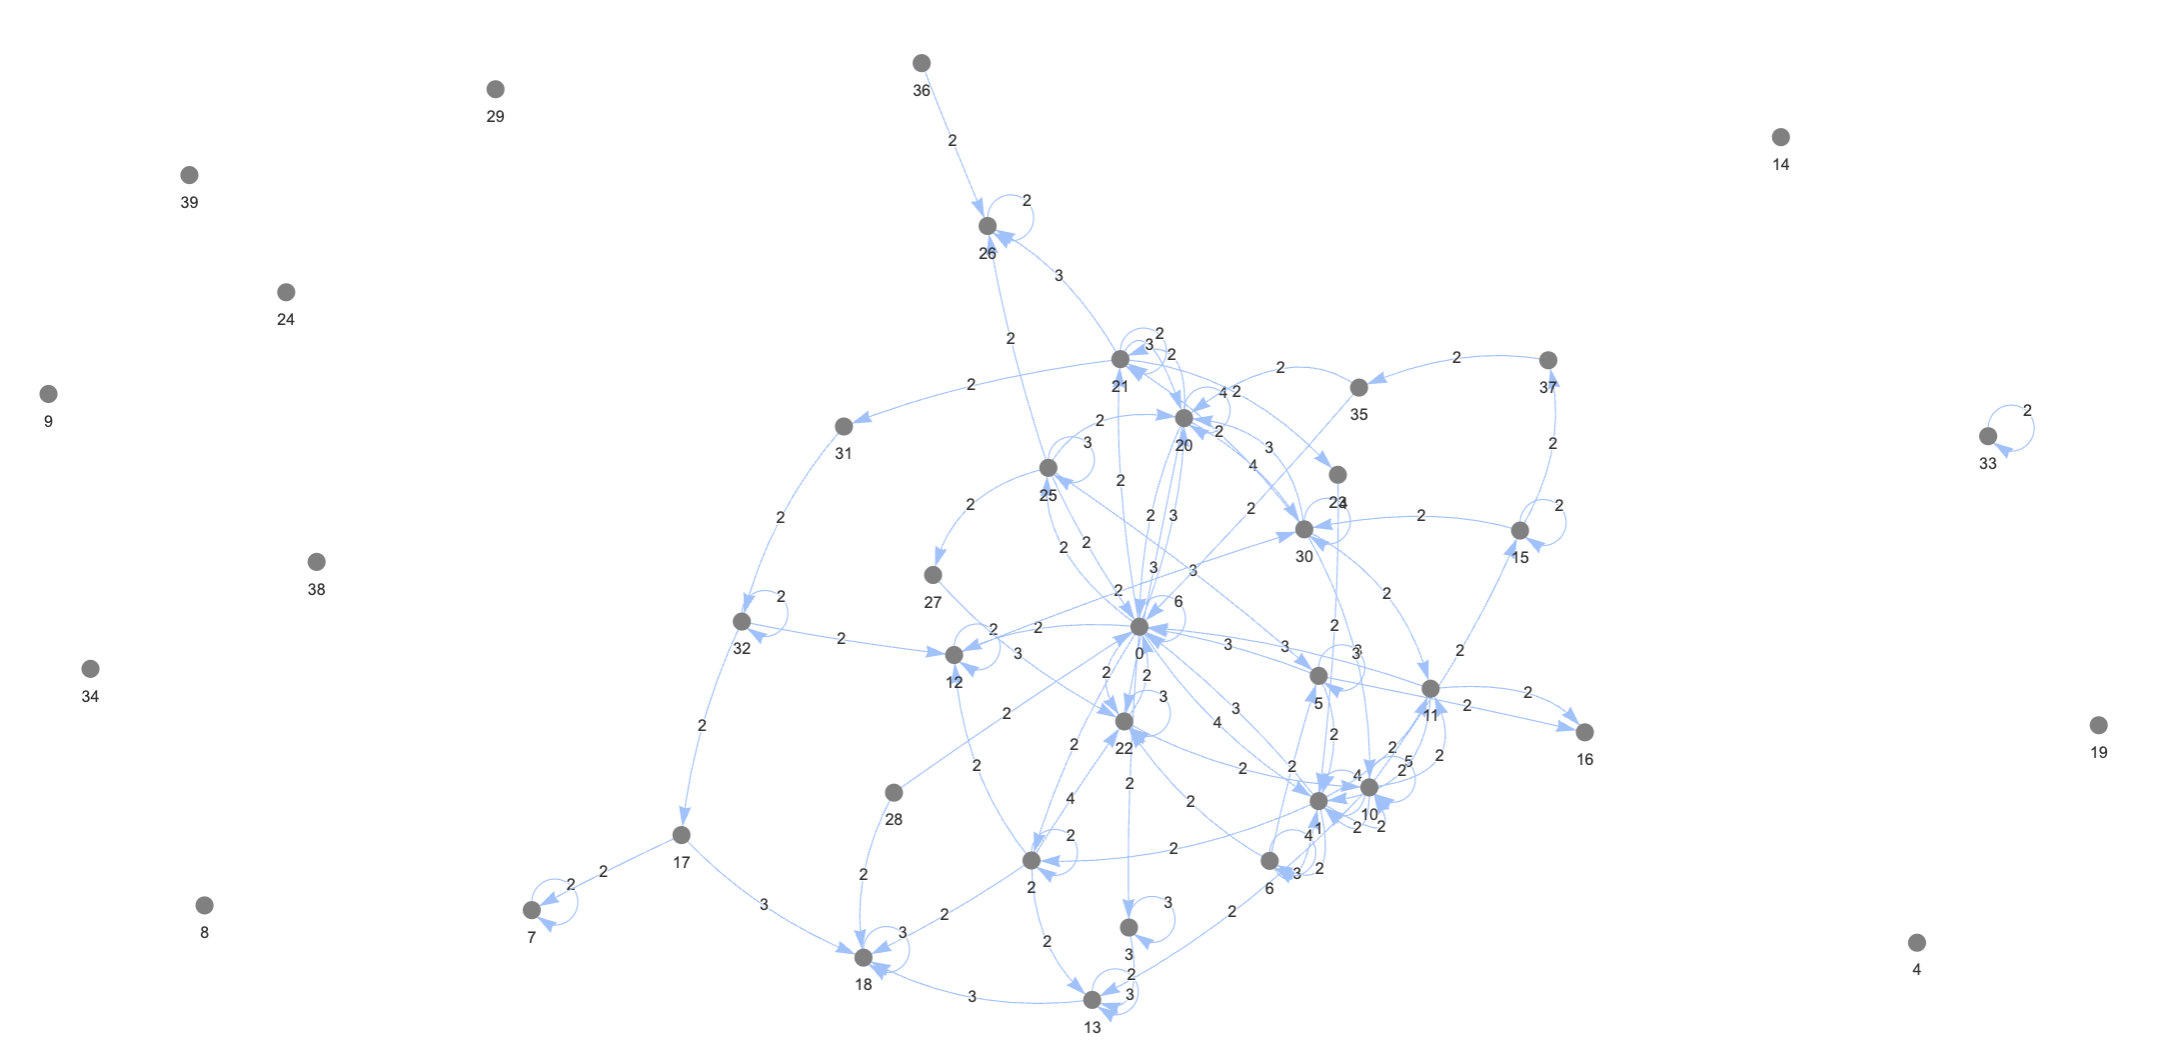
\includegraphics[width=0.40\textwidth]{rmat_graph_example_40n}
\caption{A directed, weighted R-Mat graph with $(a, b, c, d) = (0.45, 0.25, 0.25, 0.15)$, $N = 40$, $M = 400$, where edges with weight $< 2$ removed}
\label{fig:rmat_example}
\end{figure}

As parameters we will use $(a, b, c, d) = (0.45, 0.15, 0.15, 0.25)$. These are often considered the "default" parameters to generate social graphs, and fit the recommended scheme by Chakrabarti et al., the creators of this algorithm, to generate social graphs that resemble "real-world scenarios". \cite{chakrabartiRMATRecursiveModel2004, zhouKanonymityLdiversityApproaches2011} Furthermore, a common estimate for the average outdegree in a social graph is between around three and 15. Thus, we set $M = 10 \cdot N$. R-Mat graphs tend to have well-connected cores, well connected enough to turn the entire core into one, big closed delegation cycle. This is not an interesting graph to explore, since the preprocessing pipeline would collapse this core into a single node, ignoring the complex connections within the core. To avoid this, we implemented a multi-edge version of the R-Mat algorithm, which, unlike the original algorithm, places edges if happen to land in a cell that already has an edge. We then add the total amount of edges per node-pair and direction, and remove all edges where this sum adds up to less than two. This way, we define the threshold for trust that is strong enough to warrant a delegation as edges which the algorithm placed at least twice. Another important difference to the original R-Mat algorithm is that our resulting graphs are directed, whereby we simply interpret the y-axis of the adjacency matrix as the source node and the x-axis as the destination node when placing edges. \Cref{fig:rmat_example} shows an example of such a generated graph with 40 nodes.

As these graphs get pre-processed, there is no need to add any artificial sinks to the graphs, since unlike the Watts-Strogatz graphs, they do generally contain sinks. In the event of closed delegation cycles, these get collapsed into a common sink node, where all the power delegated into closed delegation cycles gets collected. In the case of these delegation graphs, we find that generally well under $1\%$ of the graph's nodes are affected by this collapse. Furthermore, the weight of the nodes is taken into account adding delegation nodes, so a node with two outdoing edges of weight two and three respectively, will end up delegating to the first node with weight 0.4 ($= \frac{2}{2+3}$), and to the second node with a weight of 0.6.

The runtimes of the algorithms on these graphs can be seen in \cref{fig:rmat}. Here, the runtimes resemble more closely those of the no-edges synthetic graphs and the runtimes of the LS and LP solver resemble the runtime they exhibited when resolving the big cycle graphs. As mentioned before, the generated R-Mat graphs contain a relatively dense community at the core, and many single nodes which neither delegate nor are delegated to. By enforcing a minimum level of trust, the amount of node in the periphery of the graph increases, since nodes which are connected to the core by just a single edge are disconnected from the core by the algorithm. Thus, only between around $7\% - 9\%$ of nodes in these graphs actually have delegations either incoming or outdoing, thus explaining why the runtimes behave very similar to how they did when the graph contained no edges at all.

\begin{figure}[t]
    \centering
    \begin{subfigure}[t]{0.45\textwidth}
        \centering
        \fbox{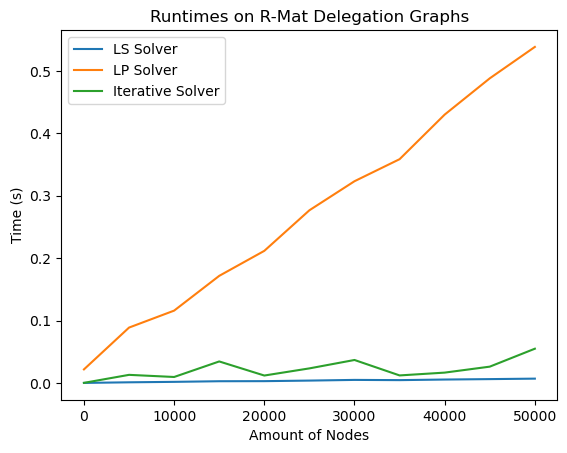
\includegraphics[width=\textwidth]{0-50000_rmat}}
        \caption{Linear scale}
        \label{subfig:rmat_linear}
    \end{subfigure}
    \hfill
    \begin{subfigure}[t]{0.45\textwidth}
        \centering
        \fbox{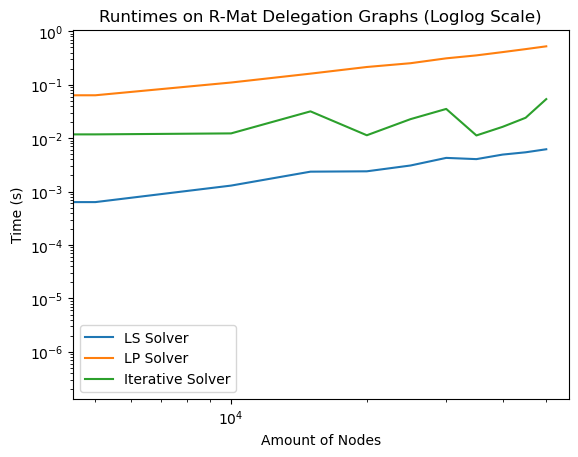
\includegraphics[width=\textwidth]{0-50000_rmat_loglog}}
        \caption{Loglog scale}
        \label{subfig:rmat_loglog}
    \end{subfigure}
    \caption{Runtimes to resolve the R-Mat based delegation graphs}
    \label{fig:rmat}
\end{figure}


\section{Real-World Datasets}

This section evaluates the three algorithms on some real-world datasets. While liquid democracy without fractional delegation has been implemented and tested in studies, to the authors knowledge there are no datasets for authentic fractional delegations. As an alternative, we have fallen back to transforming datasets which may resemble fractional delegations into delegation graphs. We  introduce the three datasets individually, followed by a joint evaluation in \cref{subsec:datasets_eval}.

\subsection{Bitcoin OTC Trust Network}

Users trading Bitcoin on the platform "Bitcoin OTC" maintain a record of trust to other users, in order to prevent transactions with untrustworthy users. SNAP provides the Bitcoin OTC Trust Graph, a graph of this trust between users. \cite{kumar2016edge, kumar2018rev2} The graph is directed and weighted, with weights ranging from -10 to 10, total distrust to total trust. 

The graph was first cleaned, to remove all edges with a non-positive trust values, before being turned into a delegation graph via the preprocessing pipeline, again not adding any sinks artificially. The preprocessing pipeline normalizes edge weights, meaning outgoing trust levels are scaled down proportionally to add up to one, preserving relative differences in trust. The finished graph contains 5573 nodes, of which about 0.15\% are sinks. The outdegree distribution in the Bitcoin OTC Trust Graph is shown in \cref{subfig:bitcoinotc_outdegrees}.

During the preprocessing of this graph, 43 of the graph's 5573 nodes were to be removed since they were in a closed delegation cycle. About 111.2 units of power were lost to closed delegation cycles,  0.02\% of the total power in the graph. The distribution of powers after resolving is shown in \cref{subfig:bitcoinotc_powers}

\subsection{Epinions}

Epinions.com is a "general consumer review site", in which members can decide whether to "trust" each other. The Stanford Network Analysis Project (SNAP) provides a web-of-trust graph generated from this relations. \cite{richardsonTrustManagementSemantic2003} The graph is directed and unweighted, thus an existing edge implies trust, and a missing edge implies the lack thereof.

After preprocessing the graph into a delegation graph, with the $n\%$ sink threshold set to zero, so the algorithm does not add any new sinks to the graph by removing outgoing edges of nodes, we observe the following statistics for the delegation graph, which will be called the Epinions Graph. The Epinions Graph contains 75139 nodes, of which about 0.21\% are sinks. \Cref{subfig:epinions_outdegrees} shows the distribution of outdegrees in the Epinions Graph, outdegree meaning the amount of outdoing edges of a node. The mean outdegree is 6.76.

330 closed delegation cycles were collapsed, which affected 740 nodes, about 0.01\% of nodes in the graph. Interestingly, most powerful node after resolving is the "lost" node, so the node where power goes, that was delegated into closed delegation cycles. The total amount of power lost adds up to 2777.056087, which accounts for about 0.037\% of power in the graph. The distribution of powers after resolving is shown in \cref{subfig:epinions_powers}.

\subsection{Slashdot Zoo}

The Slashdot technology news size has a "zoo" feature, in which users can tag other users as friends and foes. The Distributed AI Laboratory in Berlin (DAI Labor) provides a graph based on this data. \cite{kunegis2009a} It is a directed and weighted graph, where an edge weight of +1 indicates a friend relationship, and an edge weight of -1 indicates a foe relationship.

This graph was also cleaned to only contain positive edges and turned into a delegation graph, again not adding any sinks artificially. The delegation graph contains 69995 edges, of which about 0.4\% are sinks. The outdegree distribution in this graph is shown in \cref{subfig:slashdot_outdegrees}.

1061 nodes were removed due to being in a closed delegation cycle...
 
 \subsection{Evaluation of the datasets}
 \label{subsec:datasets_eval}
 
\begin{figure}[t]
    \centering
        \begin{subfigure}[t]{0.30\textwidth}
        \fbox{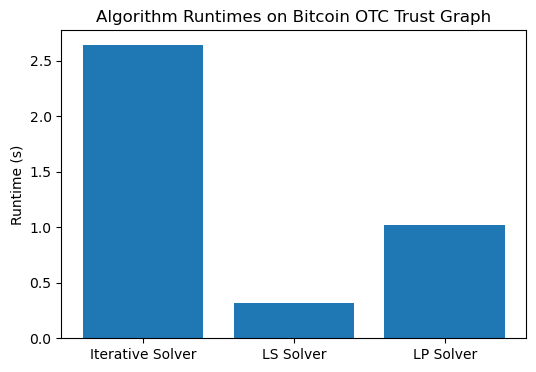
\includegraphics[width=\textwidth]{bitcoinotc_dataset}}
        \caption{Bitcoin OTC dataset}
    \end{subfigure}
    \hfill
        \begin{subfigure}[t]{0.30\textwidth}
        \fbox{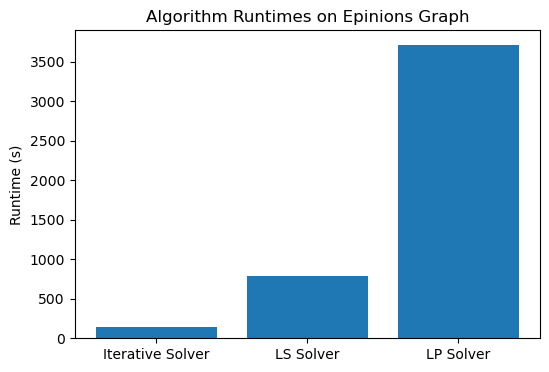
\includegraphics[width=\textwidth]{epinions_dataset}}
        \caption{Epinions dataset}
    \end{subfigure}
    \hfill
    \begin{subfigure}[t]{0.30\textwidth}
    	\centering
    	\fbox{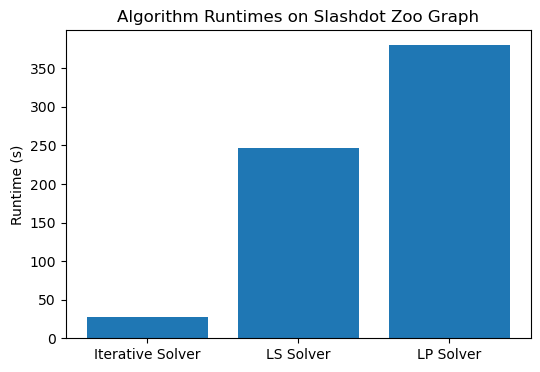
\includegraphics[width=\textwidth]{slashdot_dataset}}
    	\caption{Slashdot Zoo dataset}
    \end{subfigure}
    \caption{Runtimes}
    \label{fig:datasets_runtimes}
\end{figure}

\begin{figure}[t]
    \centering
        \begin{subfigure}[t]{0.30\textwidth}
        \fbox{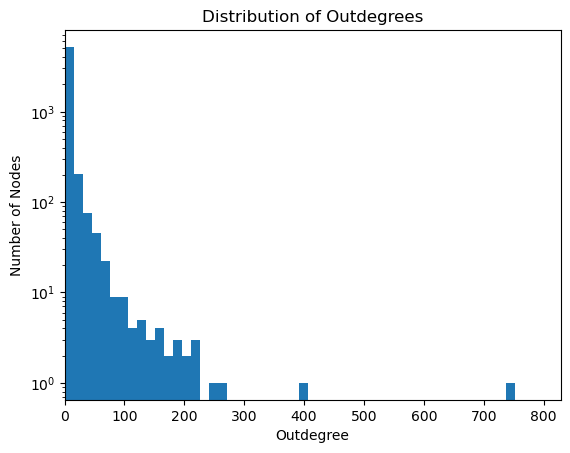
\includegraphics[width=\textwidth]{bitcoinotc_outdegree_distr}}
        \caption{Bitcoin OTC dataset}
        \label{subfig:bitcoinotc_outdegrees}
    \end{subfigure}
    \hfill
        \begin{subfigure}[t]{0.30\textwidth}
        \fbox{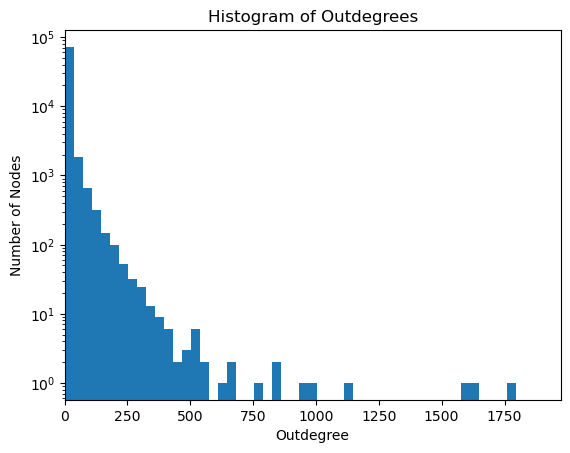
\includegraphics[width=\textwidth]{epinions_outdegree_distr}}
        \caption{Epinions dataset}
        \label{subfig:epinions_outdegrees}
    \end{subfigure}
    \hfill
    \begin{subfigure}[t]{0.30\textwidth}
    	\centering
    	\fbox{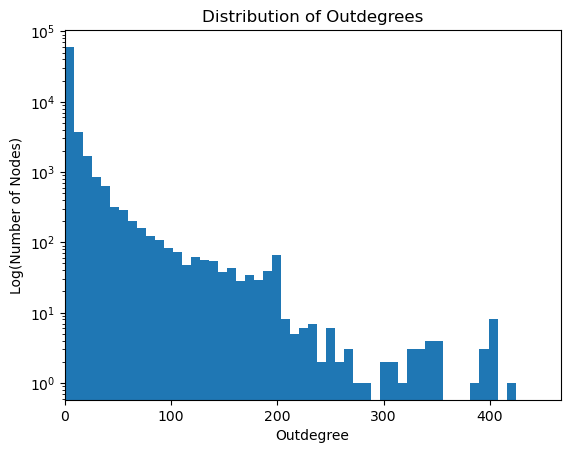
\includegraphics[width=\textwidth]{slashdot_outdegree_distr}}
    	\caption{Slashdot Zoo dataset}
	\label{subfig:slashdot_outdegrees}
    \end{subfigure}
    \caption{Histogram of outdegrees}
    \label{fig:datasets_outdegree_distr}
\end{figure}

\begin{figure}[t]
    \centering
        \begin{subfigure}[t]{0.30\textwidth}
        \fbox{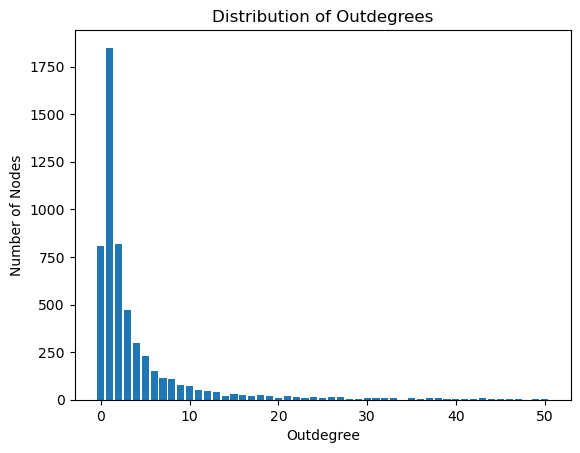
\includegraphics[width=\textwidth]{bitcoinotc_outdegree_distr_50}}
        \caption{Bitcoin OTC dataset}
        \label{subfig:bitcoinotc_outdegrees}
    \end{subfigure}
    \hfill
        \begin{subfigure}[t]{0.30\textwidth}
        \fbox{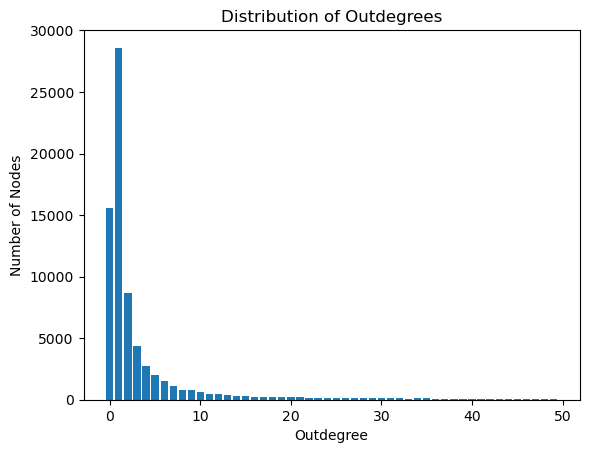
\includegraphics[width=\textwidth]{epinions_outdegree_distr_50}}
        \caption{Epinions dataset}
        \label{subfig:epinions_outdegrees}
    \end{subfigure}
    \hfill
    \begin{subfigure}[t]{0.30\textwidth}
    	\centering
    	\fbox{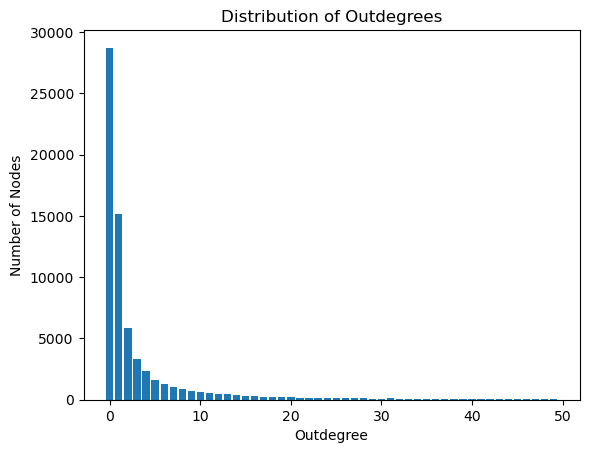
\includegraphics[width=\textwidth]{slashdot_outdegree_distr_50}}
    	\caption{Slashdot Zoo dataset}
	\label{subfig:slashdot_outdegrees}
    \end{subfigure}
    \caption{Distribution of outdegrees between 0 and 50}
    \label{fig:datasets_outdegree_distr_50}
\end{figure}

\begin{figure}[t]
    \centering
        \begin{subfigure}[t]{0.30\textwidth}
        \fbox{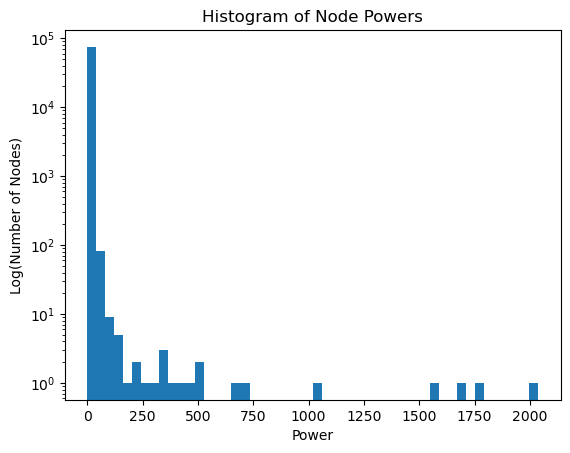
\includegraphics[width=\textwidth]{bitcoinotc_power_distr}}
        \caption{Bitcoin OTC dataset}
        \label{subfig:bitcoinotc_powers}
    \end{subfigure}
    \hfill
        \begin{subfigure}[t]{0.30\textwidth}
        \fbox{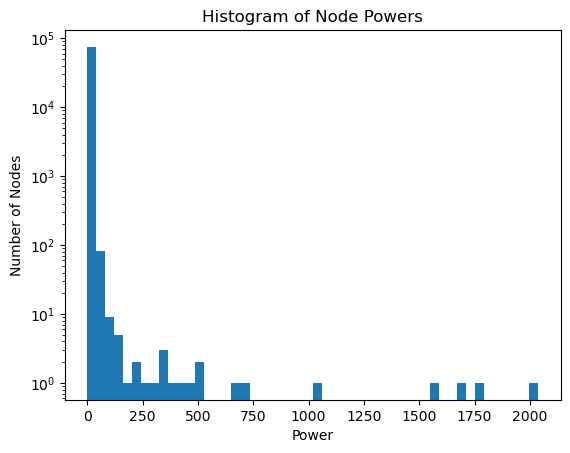
\includegraphics[width=\textwidth]{epinions_power_distr}}
        \caption{Epinions dataset}
        \label{subfig:epinions_powers}
    \end{subfigure}
    \hfill
    \begin{subfigure}[t]{0.30\textwidth}
    	\centering
    	\fbox{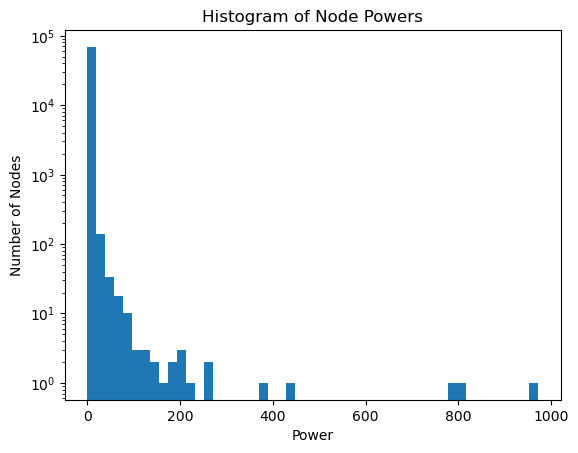
\includegraphics[width=\textwidth]{slashdot_power_distr}}
    	\caption{Slashdot Zoo dataset}
	\label{subfig:slashdot_powers}
    \end{subfigure}
    \caption{Distribution of powers}
    \label{fig:datasets_powers}
\end{figure}



The runtime results show that for the two bigger graphs, the iterative solver is the fastest, followed by the LS solver, and then the LP solver. For the Bitcoin OTC graph, the LS solver is the fastest, followed by the LP and then the iterative solver. \Cref{fig:datasets_outdegree_distr} shows histograms for the outdegrees of the three graphs. The x-axis uses a logarithmic scale, so these graphs show, that most nodes in the graphs have a rather low outdegree. \Cref{fig:datasets_outdegree_distr_50} shows, that most nodes have an outdegree of zero and one. Furthermore, histograms of the final nodes power in \cref{fig:datasets_powers} show that most nodes also have very low power values. 

Interestingly, there no nodes in either of the three datasets that have a power of exactly 1.0, suggesting that there are no isolated nodes. Despite this, the iterative solver performs the fastest on the two bigger graphs, while it is clearly outperformed in the Bitcoin OTC graph, the smallest of the three. This suggests, that this solver scales better than the other two. It can also suggest, that the Epinions and Slashdot Zoo graphs are rather free of retentive cycles. Other explanations for this low runtime can include that paths to sinks are rather short. This would mean that the algorithm does not need to iterate over the graph very often.  

\section{Key Insights}

This evaluation effectively compares three different solvers for systems of linear equations in the context of resolving delegation graphs. The investigations showed, that for smaller delegation graphs, the LS solver generally provides the best results. When graphs are very sparse or very large, the iterative solver outperforms the LS solver, however, the iterative solver is less precise than the LS solver, meaning that unless a bit of uncertainty in the power values is acceptable, the LS solver provides both great, scalable performance and perfect accuracy. When resolving large, randomly generated delegation graphs, the LS solver's runtime grew a lot faster than the LP solver's for big graphs. Also when resolving Watts-Strogatz based delegation graphs, the LS solver's runtime grew at a faster rate. However, in general the LS solver is still the more efficient choice since it generally has a faster or similar runtime growth than the LP solver, but faster runtime overall. 

\TODO{Add an annex with all the runtimes, and for some graphs where I mention extra statistics, also the data for this statistics, like amount of isolated nodes in the R-Mat discussion.}